\section{Temporal-Difference Learning}
\subsection{Exercise 6.1}
\subsubsection{Q}
If $V$ changes during the episode, then (6.6) only holds approximately; what would the difference be between the two sides? Let $V_t$ denote the array of state values
used at time $t$ in the TD error (6.5) and in the TD update (6.2). Redo the derivation above to determine the additional amount that must be added to the sum of TD errors in order to equal the Monte Carlo error.
\subsubsection{A}
Equation 6.5 becomes: $\delta_t = R_{t+1} + \gamma V_t(S_{t+1}) - V_t(S_t)$ and equation 6.2 becomes: $V_{t+1}(S_t) = V_t(S_t) + \alpha \left[R_{t+1} + \gamma V_t(S_{t+1} - V_t(S_t)\right]$. We then proceed as follows:
\begin{align}
G_t - V_t(S_t) &= R_{t+1} + \gamma G_{t+1} - V_t(S_t) + \gamma V_t(S_{t+1}) - \gamma V_t(S_{t+1}) \\
&= \delta_t + \gamma(G_{t+1} - V_t(S_{t+1})) \\
&= \delta_t + \gamma(G_{t+1} - V_{t+1}(S_{t+1})) + \gamma \theta_{t+1}, \text{with} \; \theta_{t} = \alpha \left[R_{t+1} + \gamma V_t(S_{t+1} - V_t(S_t))\right] \\
&= \delta_t + \gamma \delta_{t+1} + \gamma^2(G_{t+2} - V_{t+2}(S_{t+2})) + \gamma \theta_{t+1} + \gamma^2 \theta_{t+2} \\
&= \sum_{k=t}^{T-1} \left[\gamma^{k-t} \delta_k + \gamma^{k-t+1} \theta_{k+1}\right]
\end{align}
$
\hfill \blacksquare
$

\subsection{Exercise 6.2}
\subsubsection{Q}
This is an exercise to help develop your intuition about why TD methods are often more efficient than Monte Carlo methods. Consider the driving home example and how it is addressed by TD and Monte Carlo methods. Can you imagine a scenario in which a TD update would be better on average than a Monte Carlo update? Give an example scenario—a description of past experience and a current state—in which you would expect the TD update to be better. Here’s a hint: Suppose you have lots of experience driving home from work. Then you move to a new building and a new parking lot (but you still enter the highway at the same place). Now you are starting to learn predictions for the new building. Can you see why TD updates are likely to be much better, at least initially, in this case? Might the same sort of thing happen in the original scenario?
\subsubsection{A}
The hint above gives intuition to the answer. Let's assume we are trying to learn the optimal policy for playing a round of golf at my local course, and we assume we have already learned the value function for the course previously using monte carlo and td-learning. If 1 of the 18 holes is changed, monte carlo methods would require us to play the whole course to update our understanding of the states relating to the new hole once. With TD-learning, all we have to do is make predictions about our new hole, then we can revert to previously learned value function for the remaining holes. i.e. we bootstrap off of previous knowledge more effectively with TD-learning than monte carlo. Our convergence to the true value function using TD-learning should hence be quicker.
$
\hfill \blacksquare
$

\subsection{Exercise 6.3}
\subsubsection{Q}
From the results shown in the left graph of the random walk example it appears that the first episode results in a change in only $V(A)$. What does this tell you about what happened on the first episode? Why was only the estimate for this one state changed? By exactly how much was it changed?
\subsubsection{A}
\begin{figure}[h!]
	\centering
	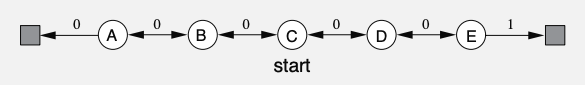
\includegraphics[width=\textwidth]{/ex6.3}
	\caption{Random walk example}
	\label{fig:ex6.3}
\end{figure}

The result of the first episode suggests the episode terminated at the left block for no reward. The value of state $A$ was updated as follows:
\begin{align}
V(A) &= V(A) + \alpha \left[R_{t+1} + V(S_T) - V(A) \right] \\
&= 0.5 + 0.1 \left[0 + 0 - 0.5\right] \\
&= 0.45
\end{align}
$
\hfill \blacksquare
$

\subsection{Exercise 6.4}
\subsubsection{Q}
The specific results shown in the right graph of the random walk example are dependent on the value of the step-size parameter, $\alpha$. Do you think the conclusions
about which algorithm is better would be affected if a wider range of $\alpha$ values were used? Is there a different, fixed value of $\alpha$ at which either algorithm would have performed significantly better than shown? Why or why not?
\subsubsection{A}
It appears from the plot the long-term accuracy of TD methods is inversely proportional to the chosen $\alpha$, which makes sense given larger alphas would cause the value function to oscillate around the true value function. It is not clear from the plot whether different values of $\alpha$ for the MC method would have increased performance as there is no concrete difference in the algorithm performance based on $\alpha$. It appears the main drawback of the monte carlo method is that it makes significantly fewer value function updates than TD methods. For 100 episodes, the MC method can make no more than 100 updates. For the TD method, the expected episode length is 6, and so it makes 600 value function updates in 100 episodes. No value of $\alpha$ can overcome the reduced sample rate.
$
\hfill \blacksquare
$

\subsection{Exercise 6.5}
\subsubsection{Q}
In the right graph of the random walk example, the RMS error of the TD method seems to go down and then up again, particularly at high $\alpha$’s. What could have caused this? Do you think this always occurs, or might it be a function of how the approximate value function was initialized?
\subsubsection{A}
As discussed above, I believe this will always occur for high $\alpha$ as the weight given to the TD error will exaggerate small errors. The will cause the estimated value function to bounce back and forth across the true value without converging. In turn, this will cause the estimate for $V(c)$ (initialised in this example at its true value) to drift away from the correct estimate, increasing RMS error.
$
\hfill \blacksquare
$

\subsection{Exercise 6.6}
\subsubsection{Q}
In Example 6.2 we stated that the true values for the random walk example are $\frac{1}{6}, \frac{2}{6}, \frac{3}{6}, \frac{4}{6}$ and $\frac{5}{6}$ for states A through E. Describe at least two different ways that these could have been computed. Which would you guess we actually used? Why?
\subsubsection{A}
\begin{enumerate}
	\item \textbf{Dynamic Programming}: we know the policy $\pi$ (take either action with $p(a) = 0.5$), and we know the transition function $p(s', r | s, a) = 1 \; \forall s,a $, thus the value of each state can be computed exactly.
	\item \textbf{First-visit monte carlo policy prediction}: set-up the state space and run simulations with our policy $\pi$. After each episode, back-prop the returns to each state and average.
\end{enumerate}

I suspect the authors used dynamic programming as it requires solving 6 trivial simultaneous equations, whereas the MC method may require thousands of episodes to converge on the true value.
$
\hfill \blacksquare
$

\subsection{Exercise 6.7}
\subsubsection{Q}
Design an off-policy version of the TD(0) update that can be used with arbitrary target policy $\pi$ and covering behaviour policy $b$, using at each step $t$ the importance sampling ratio $\rho_{t:t}$ (5.3).
\subsubsection{A}
Our TD update is:
\begin{equation}
V(s) = V(s) + \alpha \left[R_{t+1} + \gamma V(s') - V(s)\right]
\end{equation}
and our importance sampling ratio is:
\begin{equation}
\rho_{t:t} = \frac{\pi(A | S)}{b(A | S)}
\end{equation}

We assume an episode of experience is produced by our behaviour policy $b$, and the update becomes:
\begin{equation}
V_\pi(s) = V_\pi(s) + \alpha \left[\rho_{t:t} R_{t+1} + \rho_{t:t} \gamma V(s') - V(s)\right], 
\end{equation}

i.e. each update is weighted by the likelihood of the action being taken by the target policy compared to the behaviour policy, divided by sum of all previous importance samples.\\
$
\hfill \blacksquare
$
\subsection{Exercise 6.8}
\subsubsection{Q}
Show that an action-value version of (6.6) holds for the action-value form of the TD error $\delta_t = R_{t+1} + \gamma Q(S_{t+1}, A_{t+1}) - Q(S_t, A_t)$, again assuming that the values don’t change from step to step.
\subsubsection{A}
Recall, equation 6.6 was the monte carlo error written in terms of the TD error:
\begin{equation}
G_t - V(S_t) = \sum_{k=t}^{T-1} \gamma^{k-t} \delta_k
\end{equation}

We amend 6.6 as follows:
\begin{align}
G_t - Q(S_t, A_t) &= R_{t+1} + \gamma G_{t+1} - Q(S_t, A_t) + \gamma Q(S_{t+1}, A_{t+1}) - \gamma Q(S_{t+1}, A_{t+1}) \\
&= \delta_t + \gamma \left(G_{t+1} - Q(S_{t+1}, A_{t+1}) \right) \\
&= \delta_t + \gamma \delta_{t+1} + \gamma^2\left(G_{t+2} - Q(S_{t+2}, A_{t+2}\right) \\
\vdots \\
&= \sum_{k=t}^{T-1} \gamma^{k-t} \delta_k
\end{align}
$
\hfill \blacksquare
$

\subsection{Exercise 6.9}
\subsubsection{Q}
Re-solve the windy gridworld assuming eight possible actions, including the diagonal moves, rather than four. How much better can you do with the extra actions? Can you do even better by including a ninth action that causes no movement at all other than that caused by the wind?
\subsubsection{A}
\ProgrammingExercise \\

With the extra actions, the optimal policy is now 7 moves as opposed to 15 moves with 4 actions. Adding the 9th action does not improve the optimal policy, the terminal square is 7 moves away from the start square and so adding an action that keeps the agent stationary cannot improve the policy. See Figures \ref{fig:ex6.9a} and \ref{fig:ex6.9b} plot the optimal policy for 4 and 8 actions respectively. Each agent learned from 10,000 episodes of self-play.
\begin{figure}[h!]
	\centering
	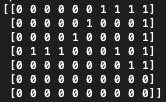
\includegraphics[width=0.5\textwidth]{/ex6.9a}
	\caption{Optimal policy with 4 available actions}
	\label{fig:ex6.9a}
\end{figure}
\begin{figure}[h!]
	\centering
	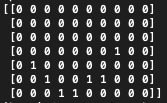
\includegraphics[width=0.5\textwidth]{/ex6.9b}
	\caption{Optimal policy with 8 available actions}
	\label{fig:ex6.9b}
\end{figure}
$
\hfill \blacksquare
$

\subsection{Exercise 6.10}
\subsubsection{Q}
Re-solve the windy gridworld task with King’s moves, assuming that the effect of the wind, if there is any, is stochastic, sometimes varying by 1 from the mean values given for each column. That is, a third of the time you move exactly according to these values, as in the previous exercise, but also a third of the time you move one cell above that, and another third of the time you move one cell below that. For example, if you are one cell to the right of the goal and you move left, then one-third of the time you move one cell above the goal, one-third of the time you move two cells above the goal, and one-third of the time you move to the goal.
\subsubsection{A}
Implementation is identical to above with amended transition function. Exercise not yet completed.
$
\hfill \blacksquare
$

\subsection{Exercise 6.11}
\subsubsection{Q}
Why is Q-learning considered an \textit{off-policy} control method?
\subsubsection{A}
Q-learning is off-policy because the action-selection at $S_{t+1}$ (used for the Q-update) is deterministic i.e. it chooses the greedy action with probability 1. This is in contrast with the behaviour policy used to collect the data which is $\epsilon$-greedy. The policy being updated is therefore different from that being used to collect data, and the algorithm is off-policy.\\
$
\hfill \blacksquare
$

\subsection{Exercise 6.12}
\subsubsection{Q}
Suppose action selection is greedy. Is Q-learning then exactly the same algorithm as SARSA? Will they make exactly the same action selections and weight updates?
\subsubsection{A}
If action-selection is greedy, the algorithms become identical, but the action selections and weight updates may differ depending on the arbitrary initialisation of $Q$ and $S$. For example, if each state-action pair is assigned a random value $Q(S, A) \in (0,1]$, the greedy action selection in each case will differ. Because action selection differs, updates differ, and because neither algorithm explore, there is no guarantee they will converge on the same solution.
$
\hfill \blacksquare
$

\subsection{Exercise 6.13}
\subsubsection{Q}
What are the update equations for Double Expected Sarsa with an $\epsilon$-greedy target policy?
\subsubsection{A}
Instead of taking the maximum action over $Q$, we continue to follow our $\epsilon$-greedy behaviour policy. The expected sarsa update is:
\begin{equation}
Q(S_t, A_t) \leftarrow Q(S_t, A_t) + \alpha \left[R_{t+1} + \gamma \sum_{a} \pi(a | S_{t+1}) Q(S_{t+1}, a) - Q(S_t, A_t) \right] \\
\end{equation}
Therefore our updates become:
\begin{align}
Q_1(S_t, A_t) &\leftarrow Q_1(S_t, A_t) + \alpha \left[R_{t+1} + \gamma \sum_{a} \pi(a | S_{t+1}) Q_2(S_{t+1}, a) - Q_1(S_t, A_t) \right]  \\
Q_2(S_t, A_t) &\leftarrow Q_2(S_t, A_t) + \alpha \left[R_{t+1} + \gamma \sum_{a} \pi(a | S_{t+1}) Q_1(S_{t+1}, a) - Q_2(S_t, A_t) \right]
\end{align}
with our policy $\pi$ being $\epsilon$-greedy.
$
\hfill \blacksquare
$

\subsection{Exercise 6.14}
\subsubsection{Q}
Describe how the task of Jack’s Car Rental (Example 4.2) could be reformulated in terms of afterstates. Why, in terms of this specific task, would such a reformulation be likely to speed convergence?
\subsubsection{A}
In Jack's car rental example we each location can hold cars in the range (0,20). Up to 5 cars can be moved from one location to the other overnight to accommodate expected sales, taking one of these actions will move us deterministically to a new state. If there was uncertainty in how we transition between states, it makes sense to learn a conventional value function that probabilistically accounts for this uncertainty, but given the transition is certain, we can learn the afterstates (the states from which we will sell the cars in the morning) and proceed.

We speed convergence by reducing the number of states to be evaluated. For example, if our state in the evening is five cars at each location: $(5,5)$ and our action is to move one car to the second location such that our morning state becomes $(4,6)$, we can evaluate this state as the same as the state-action pair of $(4,6)$ and choosing to move no cars.
$
\hfill \blacksquare
$